% Report Template
% John Godlee (johngodlee@gmail.com)
% Compile with XeLaTeX

\documentclass[a4paper, 11pt]{article}
%
\usepackage{amsmath}   % Better maths and more symbols
%
\usepackage{siunitx}
%
\usepackage{geometry}  % Set margins
\geometry{left=2.2cm,
	  right=2.2cm,
	  top=2.2cm,
  	  bottom=2cm}
\parskip 0.5cm
%\twocolumn
%
\usepackage{pdflscape} % Allow landscape pages nested in pdf
%
\usepackage{graphics}  % Insert images easily
\usepackage{graphicx}
\graphicspath{ {img/} }
\usepackage{float}  % Fancy graphics placement [H] [H!] arguments
\usepackage{subfig}
%
\usepackage{caption}
%
\usepackage{multirow}  % Table cells spanning multiple rows
%
\usepackage{enumerate}
%
\usepackage{natbib}    % Bibliography management - Use author/date citations
\bibliographystyle{agsmnourl}  % Use my custom agsm bibliography template which never includes URLs in articles
\usepackage{url}
\usepackage{cite}
%
\usepackage{lineno}
\linenumbers
%
\usepackage{eurosym}
\usepackage{textcomp}
%
\usepackage{color} 
\newcommand{\todo}[1]{\textcolor{red}{#1}}   % \todo{NOTE TO SELF WRITTEN IN RED}
%
\title{Geographically and genetically distinct populations of scots pine (\textit{Pinus sylvestris}) differ in resistance to damage by the large pine weevil (\textit{Hylobius abietis}): a common garden translocation study}
\author{John L. Godlee}


%-----------------------------------------------
\begin{document}
%-----------------------------------------------

\maketitle{}

\begin{abstract}

	Damage to coniferous tree plantation crops from the large pine weevil \textit{Hylobius abietis} causes economic losses of \euro{}140 million in Europe \textit{per annum}. Current mitigation strategies are labour intensive and only partially effective. Breeding natural resistance in host plants to insect pests has been used in many crop species to reduce damage as part of an integrated pest management strategy. Here, we conducted a common garden experiment in a previously clearfelled forestry plantation where \textit{H. abietis} are known to occur. 672 saplings, grown from seed collected from 21 naturally occurring populations of \textit{Pinus sylvestris} across Scotland were planted together in a regular grid, as is common in plantation forestry, to assess resistance to attack by \textit{H. abietis}.

	On those saplings which were attacked, we found significant variation in the total area of bark lesions between \textit{P. sylvestris} population. In contrast we found that sapling populations did not differ in their likelihood of being attacked by \textit{H. abietis}. A latitudinal pattern was observed, with saplings sourced from populations found further north being attacked more heavily than those further south. From these results it is suggested that as part of an integrated pest management strategy, planting of \textit{P. sylvestris} saplings from more southerly populations may reduce pine weevil attack in affected areas.

% between \textit{P. sylvestris} populations, suggesting that these individuals could be selected for selective breeding to produce trees that are less susceptible to \textit{H. abietis} attack at the sapling stage.

% 26\% of saplings were damaged by \textit{H. abietis} but there was no sapling mortality in the year of the study.

\end{abstract}

\section*{Introduction}

The large pine weevil (\textit{Hylobius abietis} L. Coleoptera: Curculionidae) is a common pest of newly planted coniferous tree plantations in Europe, causing damage to plantation saplings up to around five years old \citep{Ordlander1997}. Adult weevils emerge from tree stumps and feed on the bark and buds of coniferious saplings, consuming sugar rich phloem tissue \citep{Nordlander1991}. Lesions on the bark and buds of saplings (Figure \ref{damage}) as a result of feeding may cause a reduction in growth rate, stem deformation and an increased susceptibility to infection by airborne diseases of trees \citep{Leather1999}. Heavy damage may lead to stem girdling and death of the terminal growing bud resulting in a malformed trunk, limiting economic use as timber when fully grown \citep{Alfaro1989, Gill1992}. While \textit{H. abietis} may inhabit adult coniferous trees in both natural and planted coniferous forests, recently clearfelled and restocked coniferous plantation sites provide an enriched habitat for breeding \textit{H. abietis} and so pose more of a danger to planted saplings than those in naturally regenerating stands \citep{Willoughby2004, Orlander1999}. Adults lay eggs within the stumps of clearfelled trees, which are rarely removed after clearfelling, with newly emerged juvenile weevils feeding on young saplings \citep{Willoughby2004}. Planted coniferous saplings are more susceptible to \textit{H. abietis} damage than naturally regenerating saplings, probably due to water stress as a result of damage to root systems during planting \citep{Selander1990}. A single adult weevil can damage several plants over the course of a season, with \textasciitilde{}50\% sapling mortality observed across affected plantation sites in the UK and Ireland \citep{Heritage2001}. On commercial conifer plantations, \textit{H. abietis} causes annual economic losses of \euro{}140 million \textit{per annum} in Europe, of which \euro{}2.75 million (\textasciitilde{}\textsterling{}2.47 million) occurs in the UK \citep{Evans2015}. Currently, \textit{H. abietis} is the most important pest of newly planted trees in Northern Europe \citep{Evans2015}. The potential for climate change to enhance the damage caused by \textit{H. abietis}, by reducing life cycle length \citep{Leather1999} and encouraging migration into previously weevil free areas \citep{Inward2012, Barredo2015}, especially in more northerly regions, has prompted discussion of the effectiveness of current \textit{H. abietis} management practices and possible alternative methods \citep{Kapranas2017, McNamara2018}.

\begin{figure}
\centering
	\subfloat[]{
		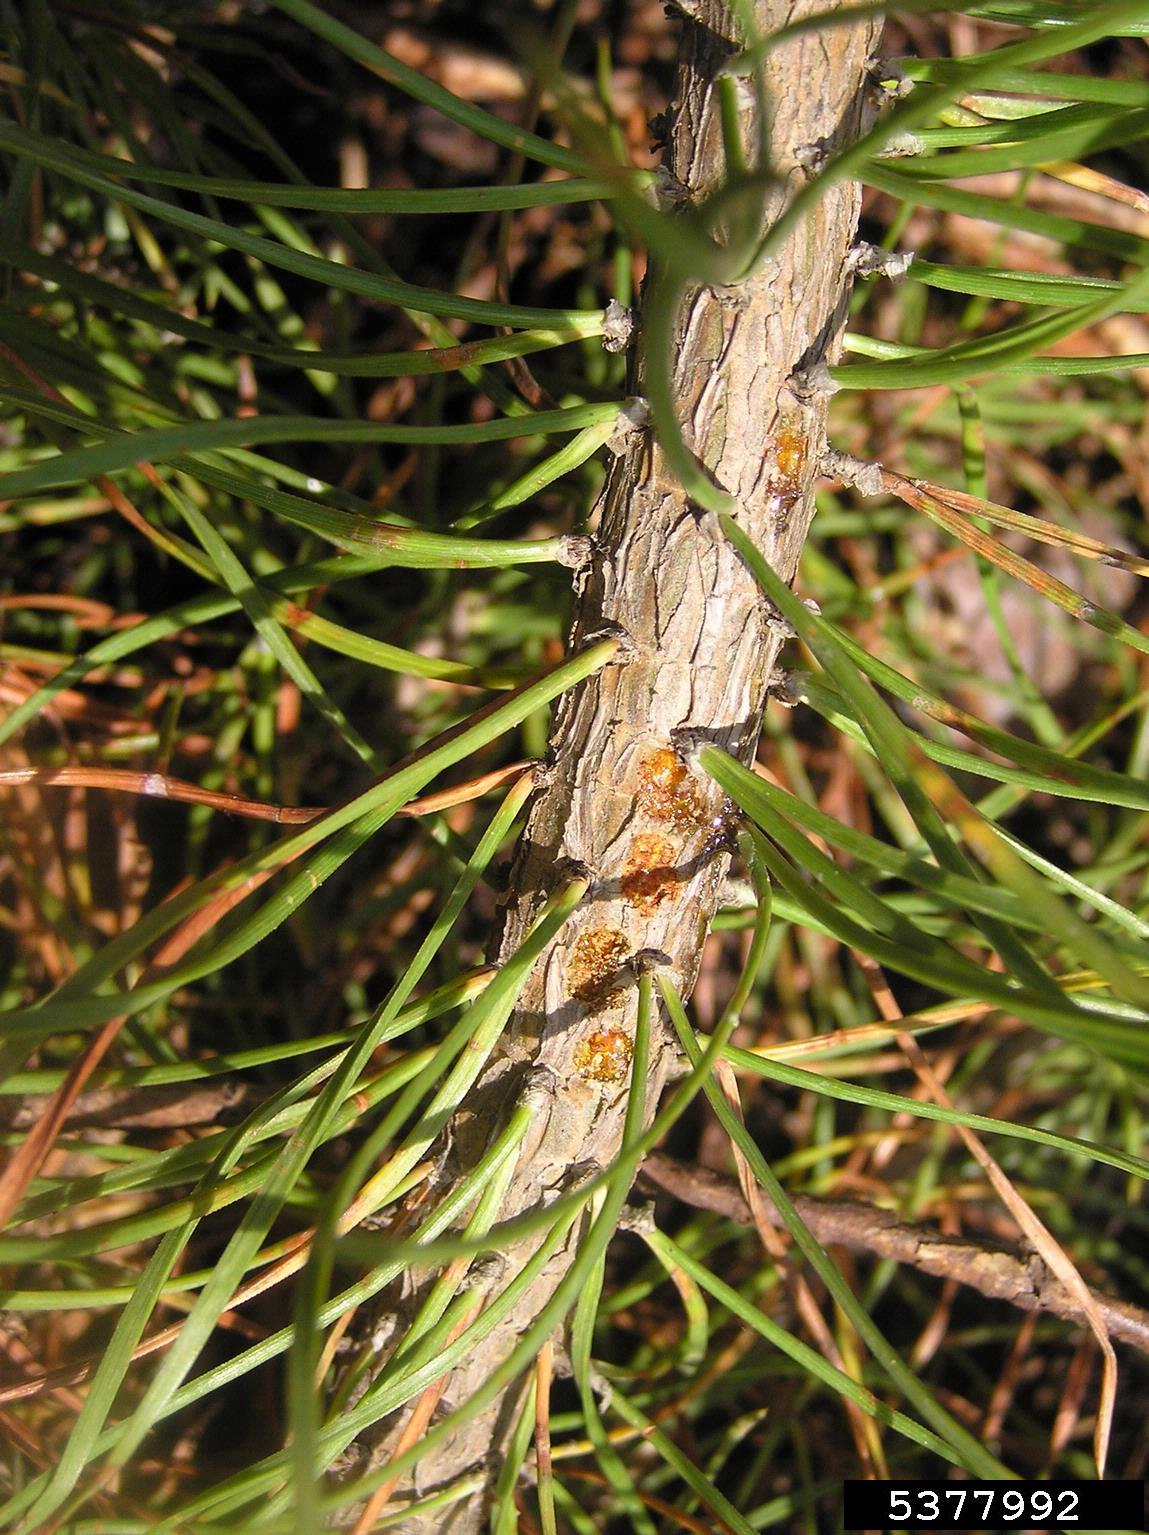
\includegraphics[width=0.4\textwidth]{damage_low} 
	}
	\subfloat[]{
		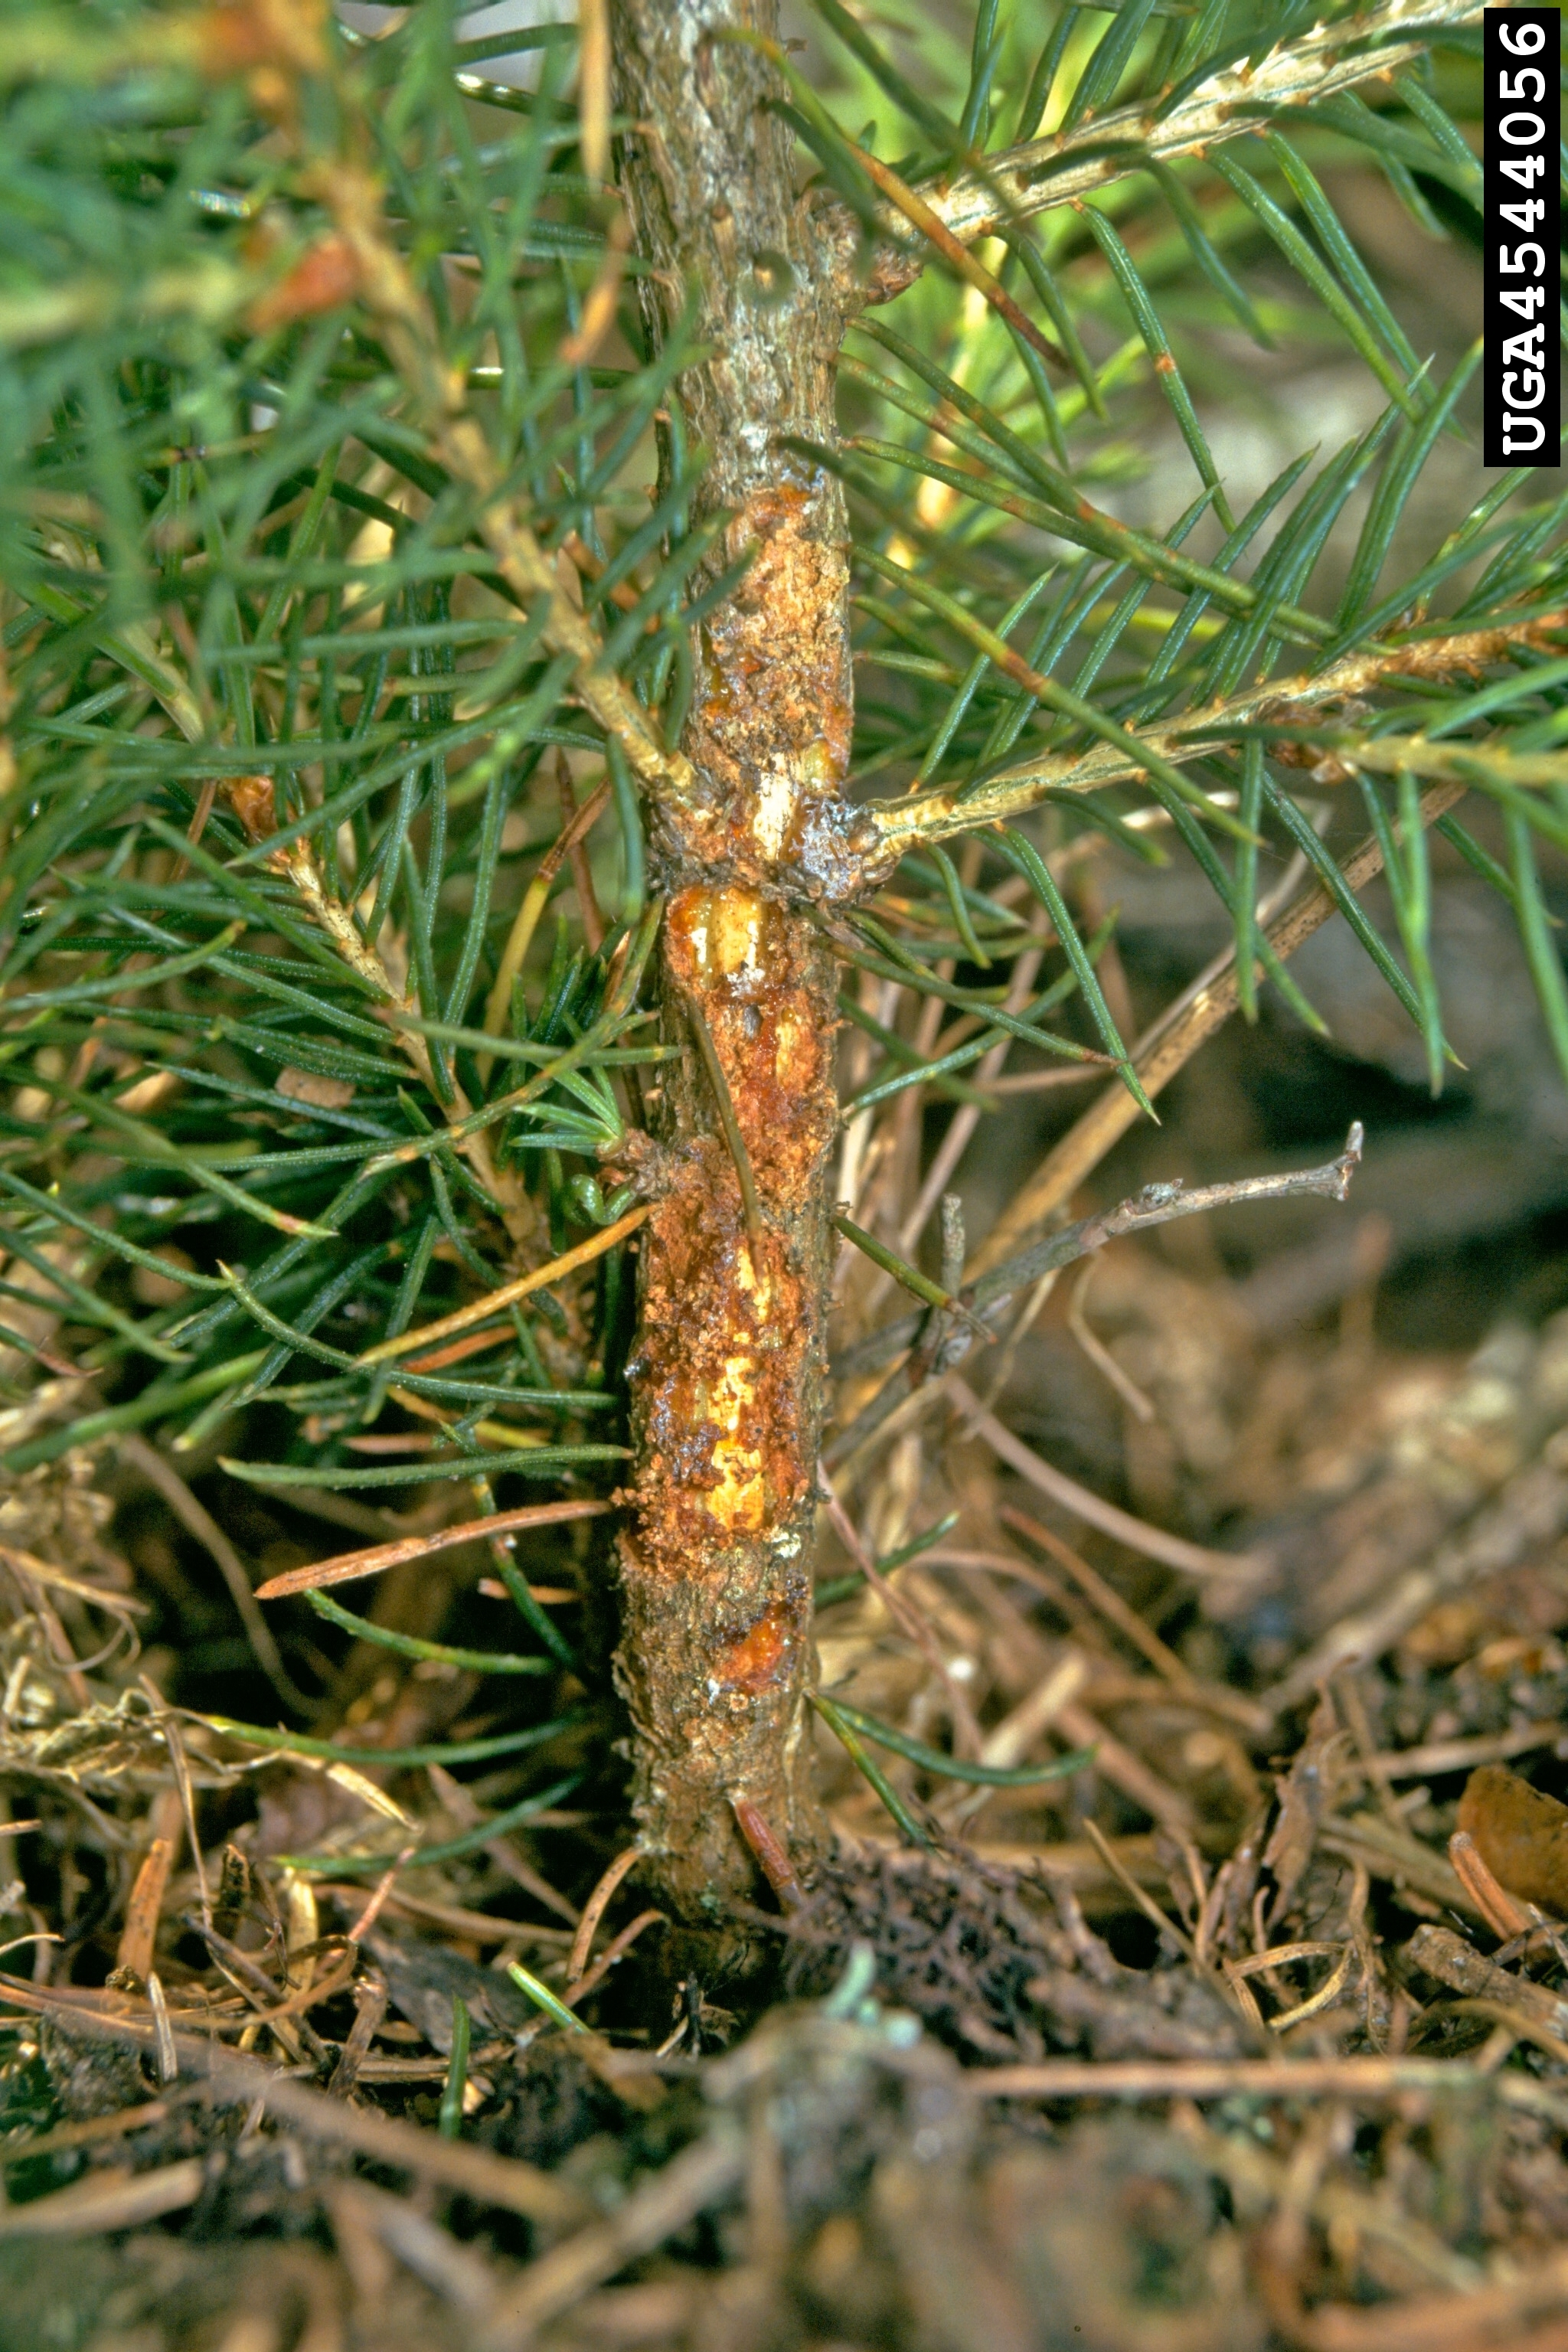
\includegraphics[width=0.4\textwidth]{damage_high}
	}
	\caption{Damage caused by \textit{Hylobius abietis}, destroying phloem tissue and causing scarring of the stem. (a) shows light damage with individual circular lesions, while (b) shows heavier damage with exposure of wood beneath the bark. Images taken from (a) Milan Zubrik, Forest Research Institute - Slovakia, Bugwood.org, and (b) Petr Kapitola, Central Institute for Supervising and Testing in Agriculture, Bugwood.org.}
	\label{damage}
% https://www.forestryimages.org/browse/detail.cfm?imgnum=4544056
% https://www.forestryimages.org/browse/detail.cfm?imgnum=5377992
\end{figure}

Management of \textit{H. abietis} currently relies on a variety of chemical, biological and physical measures, with integrated pest management schemes tending to yield greater success \citep{Willoughby2004}. Physical deterrents include piling debris produced by the clearfelling process over exposed stumps to discourage egg laying \citep{Rahman2015}, or stump removal to limit the availability of substrate for egg laying. The application of entomopathogenic nematodes after clearfelling has been shown to reduce the number of adult weevils in clearfelled sites \citep{Dillon2006, Kapranas2017, Williams2013}. The most common method of control is the addition of chemicals at the time of restocking, with \textit{H. abietis} being the only insect pest against which routine chemical controls are applied in the UK and Ireland \citep{Willoughby2004, Willoughby2017}. The most common chemical application for \textit{H. abietis} in the UK are syntehtic pyrethroids of various formulation, which are sprayed directly onto saplings as a prophylactic treatment, acting as a strong deterrent for \textit{H. abietis} feeding on treated bark \citep{Rose2005}. There are concerns however about run-off from spraying events entering watercourses, where it is highly toxic to aquatic organisms \citep{Willoughby2017, Mian1992, Antwi2015}. There are also concerns about the health of forestry workers who apply the sprays \citep{Rose2002}. Additionally, the application of pyrethroid sprays can cost \textasciitilde{}\textsterling{}80 per hectare of planted land, and requires additional top-up sprays in subsequent years if the problem persists during the sapling stage \citep{Willoughby2017}.  

\textit{H. abietis} adults rely on olfaction to search for coniferous hosts, responding to Volatile Organic Compounds (VOCs), dominated by $\alpha$-pinene and other monoterpenes released by the host plant \citep{Nordlander1986, Nordlander1987}. At the local scale, when adult \textit{H. abietis} are searching for feeding material while on the ground, after their flight muscles regress, VOCs released by open wounds on the bark caused by previous pine weevil feeders may attract more individuals \citep{Nordlander1987, Tilles1986}, worsening the damage caused to the sapling. A positive feedback mechanism may therefore exist, whereby damaged saplings are more likely to be further damaged, acting as beacons for other \textit{H. abietis} individuals. Conifer saplings may also use VOCs as a defensive strategy however, to deter insect pests \citep{Gershenzon1991, Trapp2001}. Conifer saplings may differ in the concentration of VOCs produced both prior to damage and after bark has been damaged by feeding \citep{Kivimaenpaa2012, Keeling2006}, and in their chemical composition \citep{Heijari2011} potentially causing variation in the likelihood of a sapling becoming damaged by \textit{H. abietis}. Other defensive strategies employed by coniferous tree species against insect herbivores include higher concentrations of sclereid cells in the bark and resin canals in the needles, making the plant material less palatable to herbivores, thus deterring continued feeding \citep{Donnelly2016, King2011}.

While \textit{H. abietis} is a generalist of a number of coniferous tree species \citep{Wallertz2014, Toivonen2006}, they are common pests in scots pine (\textit{Pinus sylvestris} L. Pinaceae) plantations \citep{Manlove1997}. An increasing percentage of coniferous plantation forestry in the UK is \textit{P. sylvestris}. It currently constitutes \textasciitilde{}17\% of the UK's commercial coniferous plantation forestry by area and \textasciitilde{}15\% by biomass \citep{ForestryStatistics2018}. It is one of the UK's three native coniferous tree species \citep{Cheffings2005}. There is increasing interest to plant native tree species in an attempt to preserve native biodiversity and landscape heritage. \textit{H. abietis} is the most serious pest of UK \textit{P. sylvestris} plantations, with infestations sometimes precluding sustainable future planting completely due to sapling mortality on clearfell sites \citep{Willoughby2017}.

Selective breeding and identification of \textit{P. sylvestris} varieties that are resistant to \textit{H. abietis} attack may provide a low cost method to reduce damage to saplings. Resistant varieties could form part of an integrated pest management scheme \citep{Telford2014} and planting of multiple varieties in a single forest patch could act as good insurance against potential future attacks in a rapidly changing pest landscape due to climate change \citep{Alfaro2014}. Indeed, selecting for and inducing natural resistance to \textit{H. abietis} and other bark boring insects is being heavily explored with other coniferous tree species such as \textit{Picea abies} (Norway spruce) \citep{Eyles2009, Schiebe2012}, \textit{Picea sitchensis} (Sitka spruce) \citep{King2011}, and \textit{Picea glauca} (white spruce) \citep{Kiss1991}, but \textit{P. sylvestris} has not recieved the same attention. \citet{Byun2006} found that \textit{P. sitchensis} populations varied in their expression of genes responsible for the production of bark oleoresin ducts when saplings were damaged, which act as a defence against stem boring insects. Similarly, \citet{Alfaro2013} developed varieties of \textit{P. sitchensis} resistant to the white pine weevil (\textit{Pissodes strobi} Peck Coleoptera: Curculionidae). They concluded that resin canals and sclereid cells in the bark as well as terpene production and variation in tree phenology were heritable characteristics which confer resistance to attack by \textit{P. strobi}.

Natural populations \textit{P. sylvestris} are restricted to enclaves in the north of Scotland. Remnant Caledonian pine populations in Scotland, where \textit{P. sylvestris} is the dominant species \citep{Edwards2006} are comprised of 84 fragmented woodland stands dominated by \textit{P. sylvestris}, over a total area of 17,882 hectares \citep{Mason2004}, which maintain adaptive genetic variation. Previous studies have shown that these populations vary in their ability to tolerate pathogens \citep{Perry2016} and environmental extremes \citep{Salmela2013}. This study contributes further by assessing the tolerance of natural \textit{P. sylvestris} populations to \textit{H. abietis} attack, with the hope of informing future selection of pine weevil resistant \textit{P. sylvestris} cultivars for plantation forestry, and identifying potential future conservation concerns for naturally occurring \textit{P. sylvestris} in Caledonian remnant forests. 

We conducted a common garden experiment in a recently clearfelled plantation already affected by \textit{H. abietis} with \textit{P. sylvestris} saplings in southern Scotland to assess sapling resistance to damage from the large pine weevil \textit{H. abietis}. We compared germinated seedstock collected in naturally occurring \textit{P. sylvestris} populations in remnant Caledonian pine forest patches across Scotland (Figure \ref{site_map}). We hypothesised that due to limited gene flow between Caledonian pine remnants, adaptive variation in attractiveness to \textit{H. abietis} as a food source would exist between populations of \textit{P. sylvestris}. We hypothesised that two effects contribute to the extent of damage which a sapling is subject to, based on the previous work discussed above regarding \textit{H. abietis} host searching behaviour: the probability of \textit{H. abietis} initially choosing to feed on a sapling and damaging its bark (a), and the intensity of continued feeding by \textit{H. abietis} (b). 

\section*{Materials \& Methods}

\subsection*{Study sites and species}

Scots pine (\textit{Pinus sylvestris}) is the most widely distributed pine species in the world. It's range spans Eurasia from the arctic circle in Scandinavia to the dry northern mediterranean in Spain and Turkey and from Scotland to the eastern edge of Siberia \citep{GBIF2019, Carlisle1968}. Scotland represents the western limit of its distribution, where it is the dominant canopy tree species of the Caledonian pine forest. \textit{P. sylvestris} grows well under low grazing, shade and competition. 

\textit{P. sylvestris} is wind pollinated, with monoecious flowering beginning between the ages of 15 and 30. Previous studies have shown cryptic genetic variation between the Caledonian remnant forest sites from which seeds used in this study are sourced \citep{Donnelly2018}, which supports the assertion that despite strong cross-pollination effects between the populations, some degree of genetic isolation occurs. Variation in isolatedness between sites follows a predictable longitudinal gradient, with sites on the western extreme of the Caledonian pine range being more isolated due to the prevailing easterly wind direction limiting pollen dispersion to the west \citep{Gonzalez2018}. 

Seed populations of \textit{P. sylvestris} were collected from 21 sites where genetic variation has already been identified across Scotland in March 2007 (Figure \ref{site_map}). At each site four open-pollinated trees were located at least 100 m apart. From each of these trees at least 20 cones with seeds were collected. To minimise seedling mortality, seeds were germinated and grown in a glasshouse for 3 years before four randomly selected surviving seedlings per parent tree were transplanted to a common garden. This resulted in 168 distinct maternal lines. All seed was collected from old adult trees, in an attempt to avoid sampling trees descended from nearby plantation forestry as this study focussed only on natural populations. Sites were situated within the historical range of the Caledonian pine forest. Seed collection sites were chosen by accessibility in six geographic clusters. Each cluster was located to ensure geographical isolation from others. 

\begin{figure}
	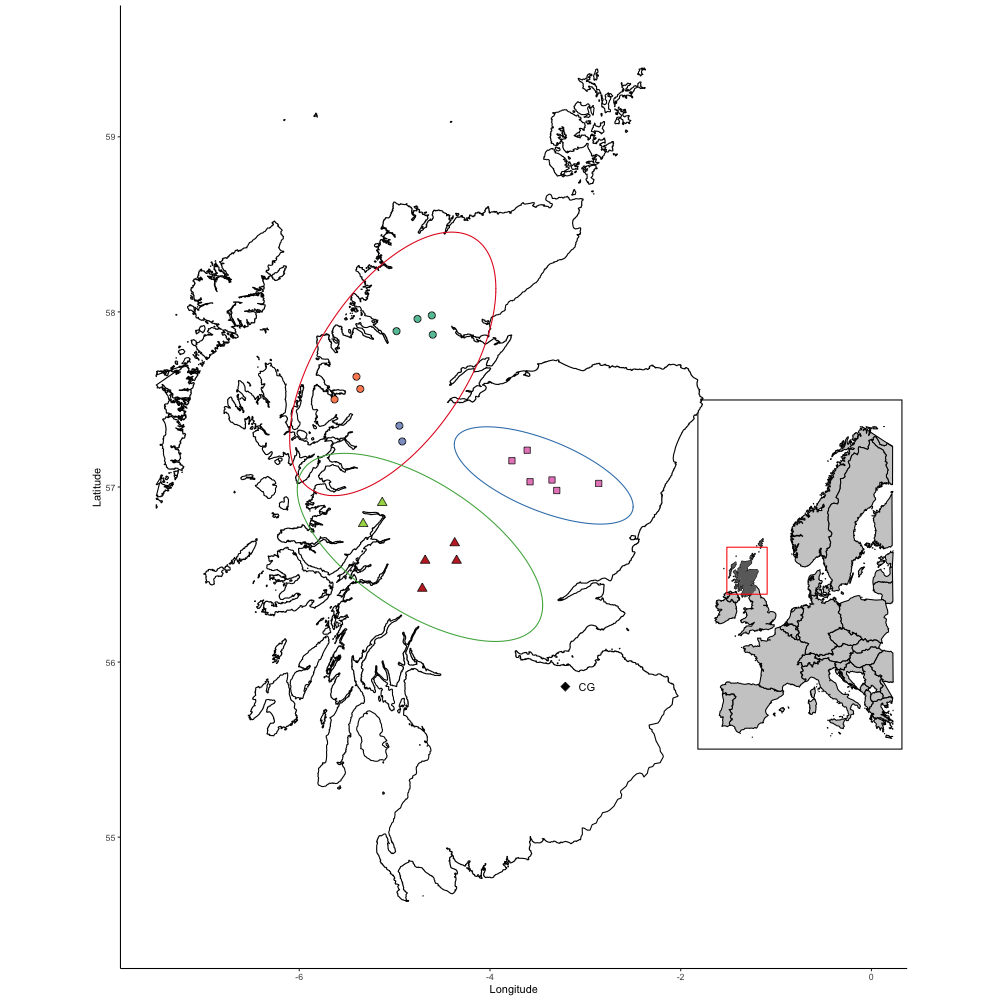
\includegraphics[width=\textwidth]{site_map}
	\caption{Map of seed collection sites within Scotland, from which seed populations were collected. Elliptic hulls and site point shapes define the three Regional zones. Points are coloured according to Geographic zone clusters, which are nested within Regions.} 
	\label{site_map}
\end{figure}

\subsection*{Experimental design}

The common garden was located in Southern Scotland (N 55.86\textdegree{}, E \textminus{}3.21\textdegree{}) in a patch of recently clear-felled sitka spruce (\textit{Picea sitchensis}) plantation, surrounded by existing adult \textit{P. sitchensis} plantation on all sides. This mimicks the conditions found in commercial plantation forestry sites that will be replanted, which often have adjacent existing plantation. A mown grass border of 10 m on all sides separated the newly planted \textit{P. sylvestris} from the surrounding \textit{P. sitchensis} plantation, to avoid competitive edge effects. All \textit{P. sitchensis} surrounding the common garden was planted at the same time in 2005, making it 10 years old when the common garden was established. %Planting was divided into four blocks of equal size running perpendicular to the average slope of the site. Each block contained 167 saplings, with saplings placed in a grid pattern within each block, with a gap between each sapling of \todo{METRES} and between saplings and the plot edge \todo{FIGURE REF}. 
Saplings were randomly assigned to grid points within 4 adjacent blocks with a distance of 3 m between each sapling. This resulted in a total grid size of 84 x 8 saplings, a total of 672 saplings. \textit{H. abietis} infestation occurred naturally across the site, with adult weevils likely travelling from the adult \textit{P. sitchensis} plantation around the common garden. 

\subsection*{Data collection}

The area of bark lesions caused by \textit{H. abietis} was counted on each sapling stem in July 2015. This is roughly between the two seasonal peaks of weevil feeding that are commonly observed in the UK, which occur in the spring and late summer, coinciding with the end of adult hibernation and the emergence of new adults from pupae, respectively \citep{Nordenhem1989, Leather1999}. Only damage sustained by \textit{H. abietis} during the current growing season was counted and could be clearly separated from damage sustained in previous years by the lack of bark edge scarring and presence of sap at the wound edge (Figure \ref{damage}). Isolated lesions tended to be roughly circular with a diameter of \textasciitilde{}3 mm. Where a larger continuous lesion was found, as when a stem was girdled, the larger lesion was photographed with a scale and the area estimated by tracing the lesion with ImageJ version 1.50g7 \citep{Schneider2012}. Weevil damage is therefore expressed as the mm\textsuperscript{2} area of stem lesions per sapling. 

\subsection*{Statistical analysis}

To assess the effect of sapling genetic origin on damage by pine weevils, and to test our hypothesis that two effects are responsible for \textit{H. abietis} damage, we implemented a hurdle model framework with generalised linear mixed models, using the \textit{glmmTMB} package in R \citep{glmmTMB}. First, a binomial logistic mixed effects regression assessed variation in the probability of a sapling being initially damaged  according to \textit{P. sylvestris} parent population. The response variable of this model was binomial, describing whether an individual sapling had experienced any damage by \textit{H. abietis}. Then a linear mixed effects model using data only saplings where damage had occurred, assessed whether saplings varied in the total area of bark damaged by continued feeding by \textit{H. abietis} according to \textit{P. sylvestris} parent population. The response variable of this model was the area of weevil damaged bark visible on the sapling. Area of bark damaged was log transformed in order to better meet model assumptions. In both analyses, parent tree was used as a random intercept effect to account for pseudo-replication in sapling parent. The nested geographic nature of the seed collection sites was also used as a random effect, with site nested within geographic zone (Figure \ref{dendro}). All statistical analyses were performed in R version 3.4.2 \citep{RCoreTeam2019}. Model goodness-of-fit was assessed for both model types by comparing models with equivalent random effects models and null models using AIC\textsubscript{r} (Akaike Information Criterion) and Log-likelihood estimates \citep{Bolker2008}. During model comparison all models were fitted using Maximum Likelihood (ML) \citep{Bolker2008}. To investigate which populations of \textit{P. sylvestris} differed in their resistance to \textit{H. abietis} attack, the models were refitted using Restricted Maximum Likelihood (REML) and model slope estimates were compared. Tukey's HSD multiple comparisons test assessed which populations were significantly different from each other for both models, using the \todo{PACKAGE} package \citep{}.

Spatial autocorrelation in area of bark damaged due to damaged saplings acting as olfactory beacons to attract weevils was investigated using Generalised Least Squares (GLS) models of damaged bark area with spatial autocorrelation structures as a covariate. Multiple spatial autocorrelation structures were tested and models fitted using ML were compared in their goodness-of-fit using AIC (Akaike Information Criterion) values, Log-likelihood estimates and pseudo R-squared model values calculated by the \textit{MuMIn} package \citep{MuMIn}. After model selection, the best generalised least squares model was re-fitted using REML for model interpretation to assess the predictive effect of spatial auto-correlation on weevil damage. Semi-variograms of the best fitting model residuals and raw damaged area mm\textsuperscript{2} data confirmed that spatial autocorrelation between saplings was negligible within the common garden and so spatial autocorrelation structures were not included in other models.

\section*{Results}

\subsection*{Sapling damage}

36.9\% (248/672) of the saplings in the common garden were damaged by \textit{H. abietis} feeding activity. Figure \ref{barchart} shows the number of saplings damaged divided into seed collection site populations. All saplings were alive prior to data collection and sapling mortality was not recorded during the experiment. All seed populations had at least eight affected saplings out of a total of 32. The population with the highest number of damaged saplings was Loch Clair (LC), which had 18 damaged saplings. The sapling with the highest mm\textsuperscript{2} damaged area was from Cona Glen (CG) and had 325.8 mm\textsuperscript{2} of bark damaged. Rhidorroch (RD) had the highest cumulative damaged area with 1057.1 mm\textsuperscript{2}. Variation in bark area damaged within seed populations was high (Figure \ref{boxplot}), with some geographic zones having similar levels of damage while others varied a great deal within geographic zone.

\begin{figure}
	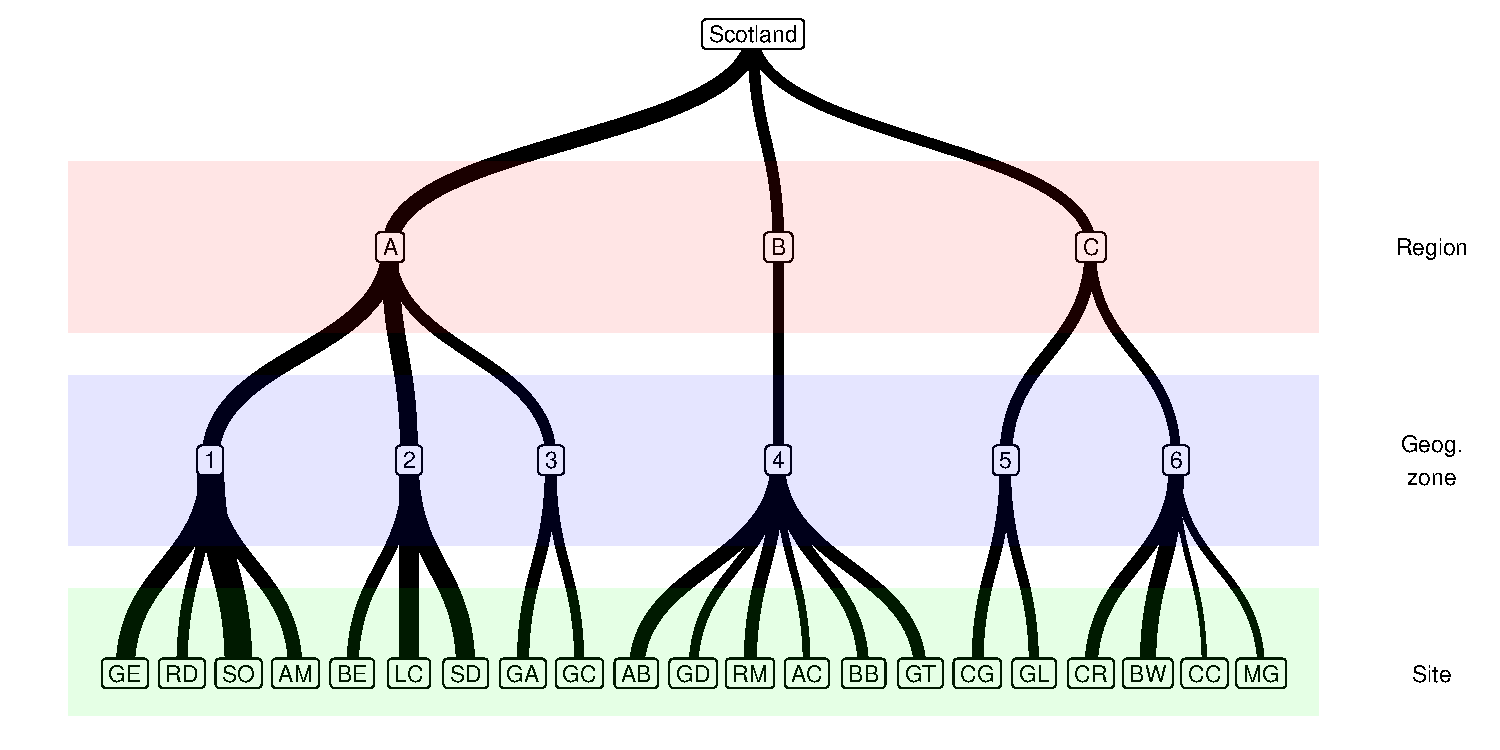
\includegraphics[width=\textwidth]{dendro}
	\caption{Dendrogram showing nested grouping of seed populations. Graph edge widths vary relatively according to the total bark area damaged on saplings collected from each site. Width edges are weighted according to the number of saplings at each grouping level to account for differences in number of sites per Geographic zone and Regional zone. This means edge widths should not be compared across vertical node levels.}
\end{figure}

\begin{figure}
	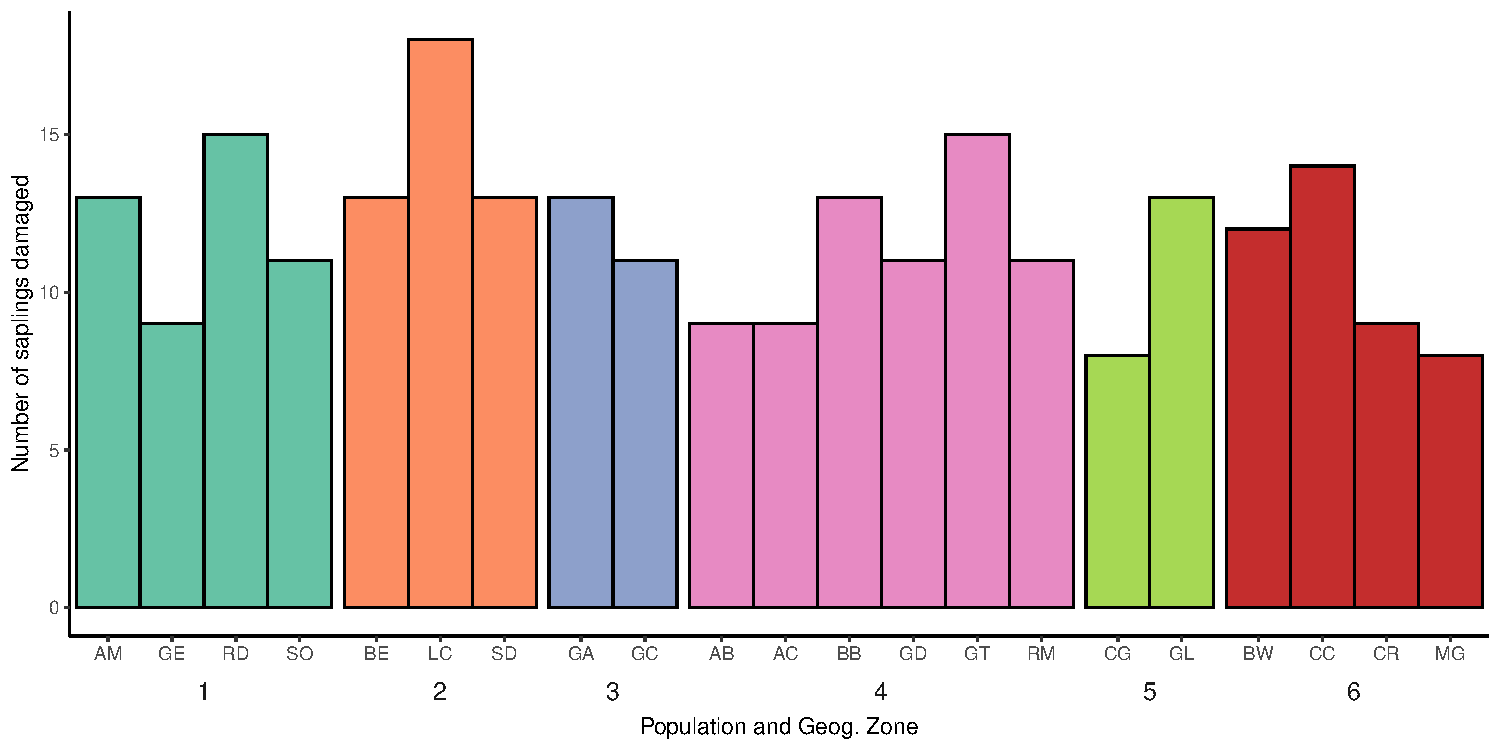
\includegraphics[width=\textwidth]{barchart}
	\caption{The number of saplings with visible damage by \textit{H. abietis}, divided by seed population. Groups of bars denote Geographic zones.}
	\label{barchart}
\end{figure}

\begin{figure}
	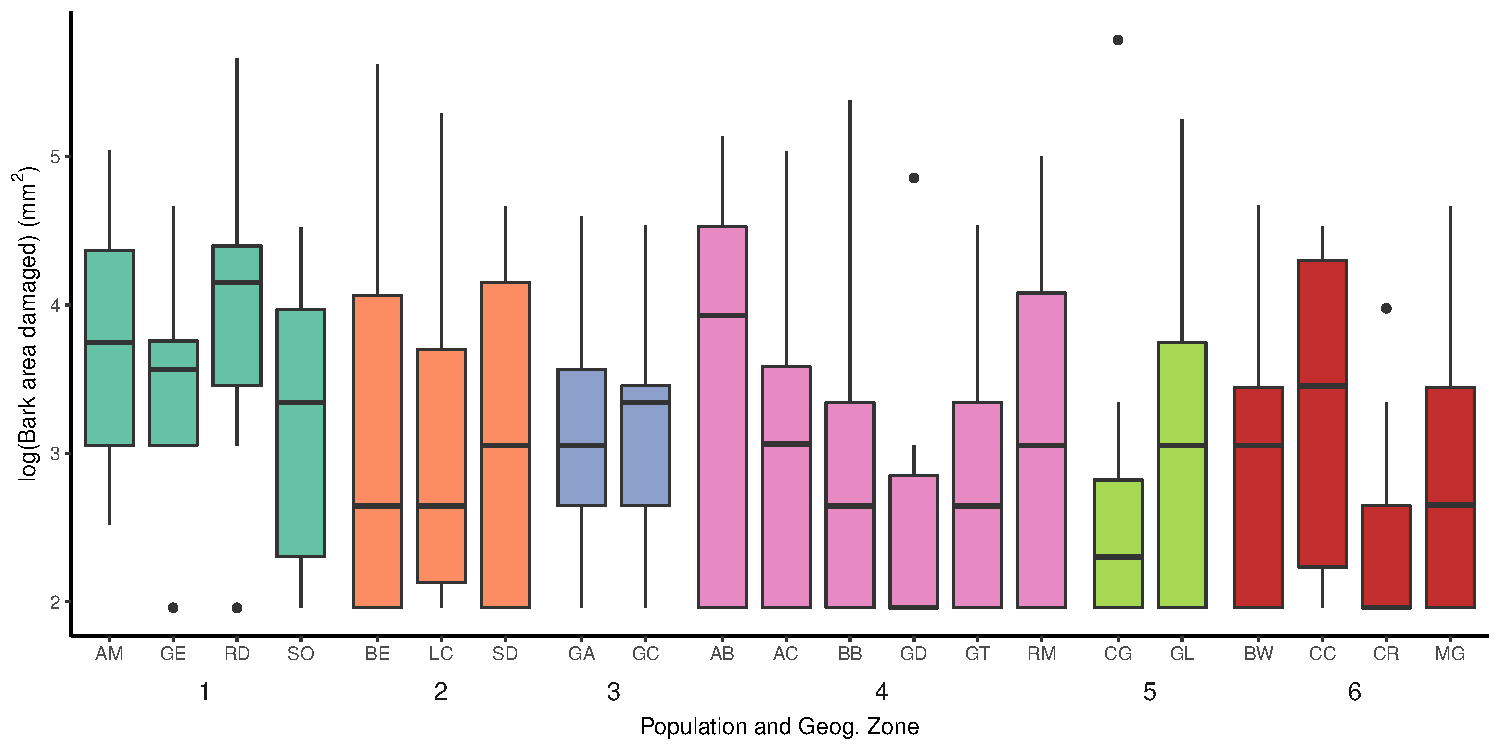
\includegraphics[width=\textwidth]{boxplot}
	\caption{Variation in bark area damaged by \textit{H. abietis}, divided by seed population. Coloured groups of bars denote Geographic zones. Thick bars denote the median value per population.}
	\label{boxplot}
\end{figure}


\subsection*{Spatial autocorrelation}

Multiple Generalised Least Squares (GLS) models of damaged sapling area fitted with different correlation structures were compared against a null model with no correlation structure using AIC values (Table \ref{cor_table}). A Gaussian correlation structure fit the data best, but explained only a very low percentage of the variation in sapling damaged area. Gaussian, Exponential and Rational quadratic models had AIC values within 2 points of each other and explained only negligibly different amounts of variation in damaged bar area, according to pseudo-R\textsuperscript{2} model values, so these models can be interpreted as fitting the data similarly well. All three models were better than a null model which explained none of the variation in damaged bark area. A semivariogram of damaged bark area with distance between saplings showed that there was no appreciable spatial auto-correlation (Figure \ref{semivariogram}). This was supported by a visual inspection of a schematic map of damaged bark area per sapling in the common garden (Figure \ref{sapling_map}). As a result, further modelling with mixed effects models did not include a spatial auto-correlation covariate structure.

\begin{figure}
	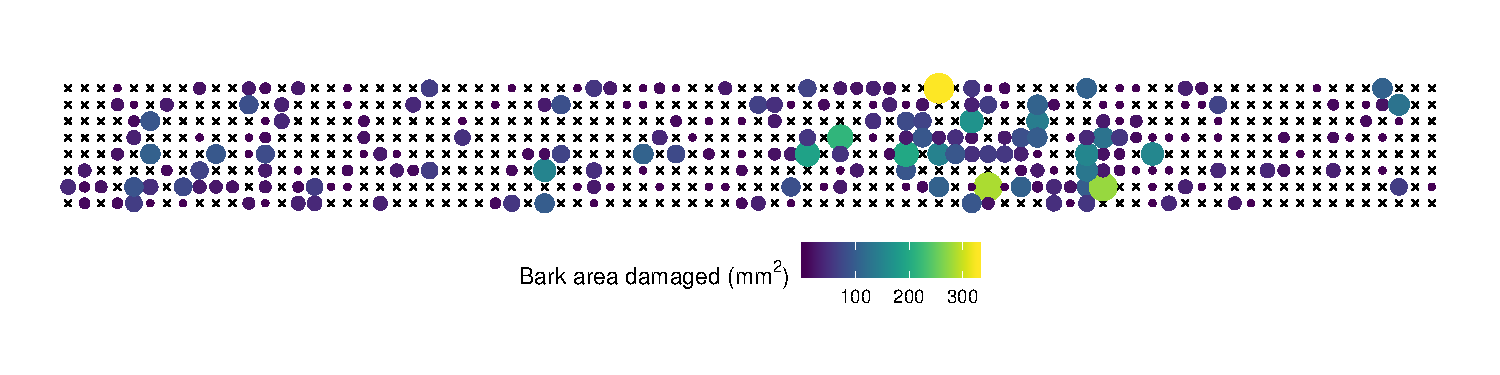
\includegraphics[width=\textwidth]{sapling_map}
	\caption{Schematic diagram of sapling relative position within the Common Garden, with sapling points coloured and sized according to the area of bark damaged. The distance between saplings is 3 m in both the X and Y directions.}
	\label{sapling_map}
\end{figure}

\begin{figure}
	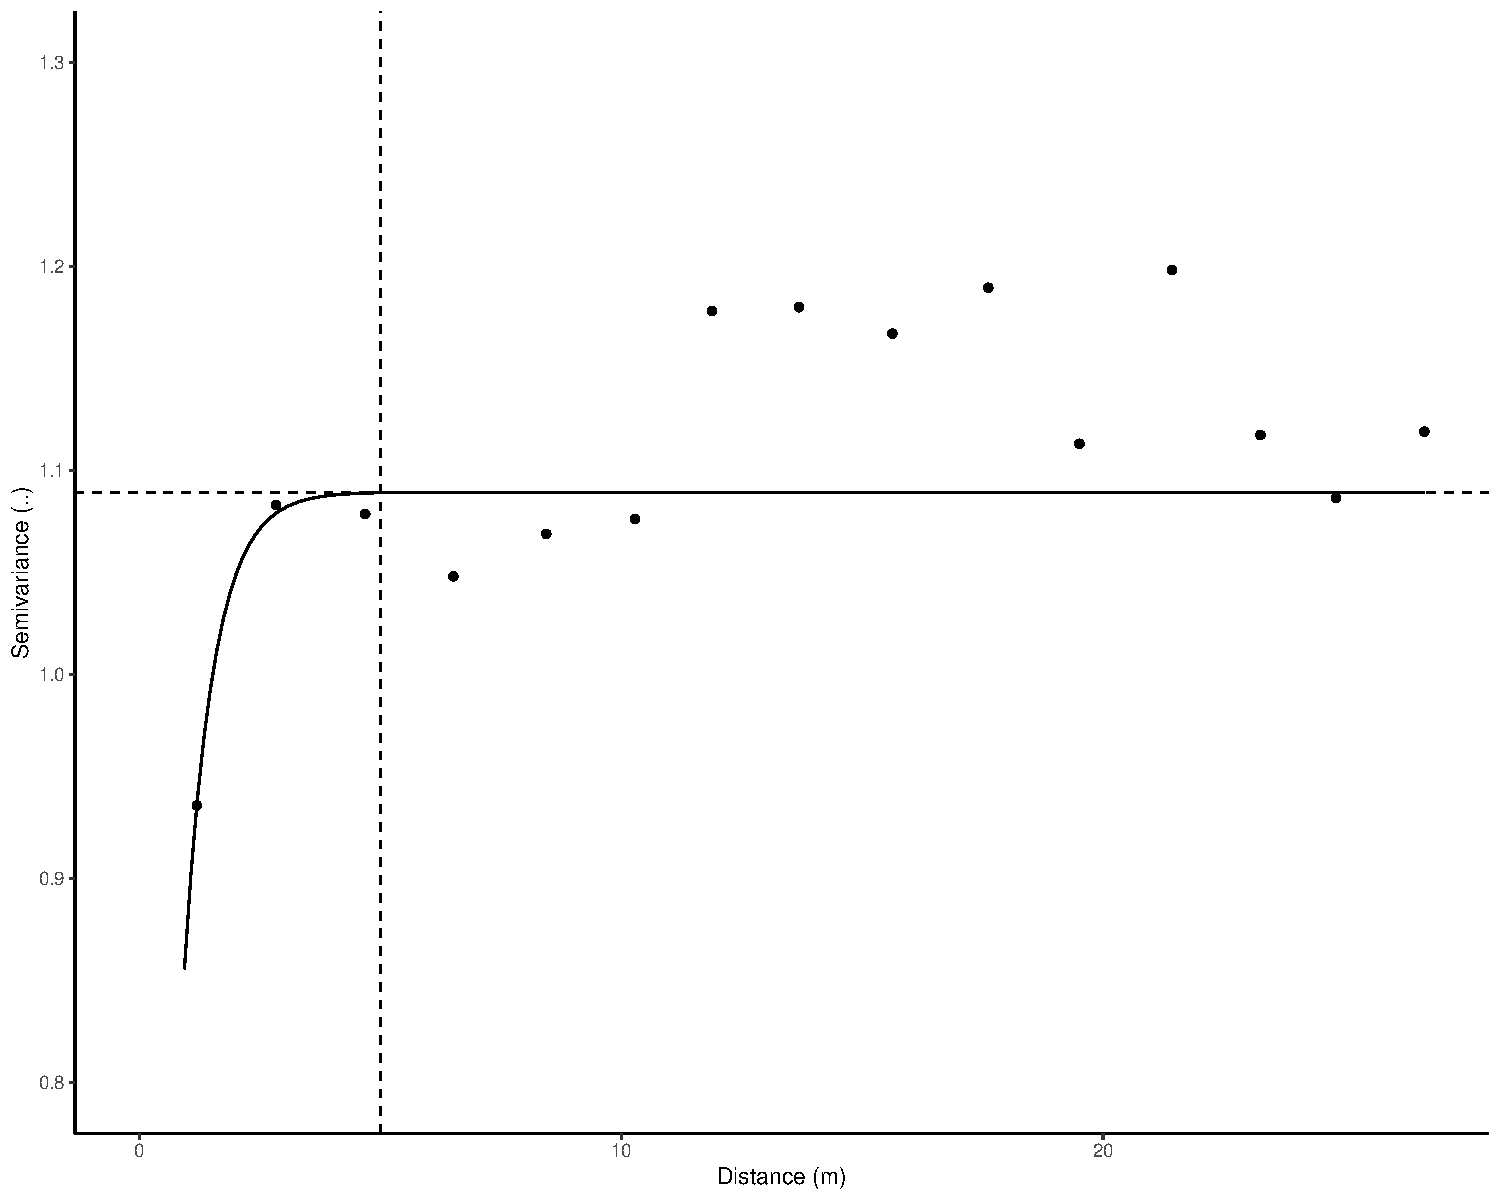
\includegraphics[width=\textwidth]{semivariogram}
	\caption{Semivariogram showing spatial autocorrelation of damaged bark area according to distance between saplings. Vertical dotted line denotes the nugget and the horizontal dotted line denotes the sill of the semivariogram.}
	\label{semivariogram}
\end{figure}

\begin{table}
  \centering 
  \caption{Model comparison of Generalised Least Squares models predicting damaged sapling bark area using different spatial autocorrelation structures. Models are ordered by increasing AIC value.} 
  \label{cor_table} 
\begin{tabular}{@{\extracolsep{5pt}} lS[table-format=3.2]S[table-format=3.2]S[table-format=3.2]} 
\\[-1.8ex]\hline 
\hline \\[-1.8ex] 
Correlation Structure & {AIC} & {Log Likelihood} & {Pseudo R\textsuperscript{2}} \\ 
\hline \\[-1.8ex] 
Gaussian & 719.573 & -355.786 & 0.033 \\ 
Exponential & 720.306 & -356.153 & 0.031 \\ 
Rational quadratic & 720.496 & -356.248 & 0.028 \\ 
Null & 725.404 & -360.702 & 0.000 \\ 
Spherical & 728.224 & -360.112 & 0.004 \\ 
Linear & 728.224 & -360.112 & 0.004 \\ 
\hline \\[-1.8ex] 
\end{tabular} 
\end{table} 

\subsection*{The effect of seed population on sapling damage}

The first part of the hurdle model process explored variation among seed populations in the probability of a sapling being damaged by \textit{H. abietis}. The most parsimonous fixed effects model included the fixed effect of geographic zone rather than individual populations (Table \ref{binomial_comp}), but only accounted for a very small percentage of the variance in the likelihood of a sapling being damaged (R\textsuperscript{2}\textsubscript{m} = 0.008) and was less parsimonious than an equivalent random effects model ($\Delta$AICr = 7.51). The models with the greatest explanatory power included maternal parent as a fixed effect and Geographic zone and seed population as nested random intercept effects. These models explained \textasciitilde{}95\% of the variance in the likelihood of a sapling being attacked, but almost all of this was due to the random effects structure (\textasciitilde{}94\%).

\begin{figure}
	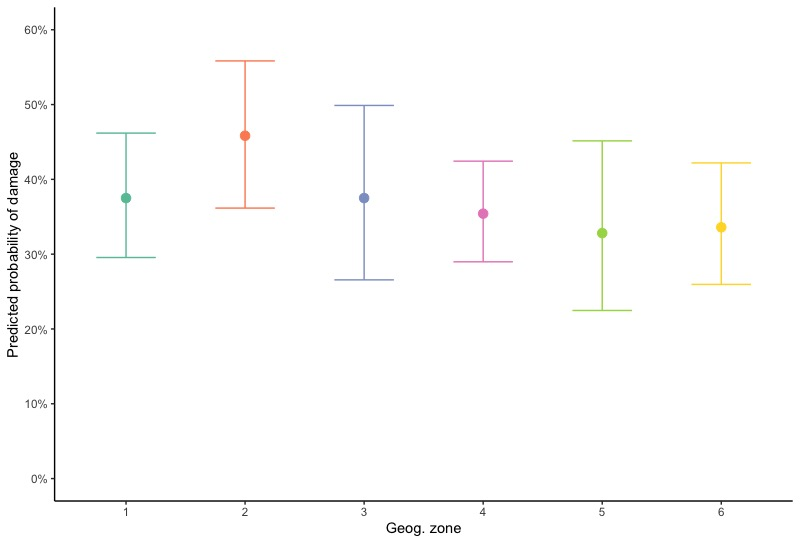
\includegraphics[width=\textwidth]{pred_binom}
	\caption{Predicted values with 95\% confidence intervals for the probability of a sapling being damaged with seed collected from different Geographic Zones.}
\end{figure}

\todo{Look at which populations are the most different}

\todo{How strong was the effect of population?}

\begin{table}[!htbp]
  \caption{Model comparison of logistic generalised linear mixed effects models predicting the likelihood of a sapling being attacked by \textit{H. abietis}. Models are sorted according to increasing AIC.} 
  \label{} 
\centering
\begin{tabular}{@{\extracolsep{5pt}} llS[table-format=3.2]S[table-format=3.2]S[table-format=3.2]S[table-format=3.2]} 
\\[-1.8ex]\hline 
\hline \\[-1.8ex] 
Fixed eff. & Random eff. & {AIC} & {logLik} & {R\textsuperscript{2}\textsubscript{m}} & {R\textsuperscript{2}\textsubscript{c}} \\ 
\hline \\[-1.8ex] 
NA & NA & 886.953 & -442.476 & 0 & 0 \\ 
NA & Site & 888.953 & -442.476 & 0 & 0 \\ 
NA & Site / Family & 890.953 & -442.476 & 0 & 0 \\ 
NA & Geog. zone / Site / Family & 892.953 & -442.476 & 0 & 0 \\ 
Geog. zone & Site & 894.462 & -440.231 & 0.008 & 0.006 \\ 
Geog. zone & Site/Family & 896.462 & -440.231 & 0.008 & 0.006 \\ 
Site & Family & 910.721 & -433.361 & 0.035 & 0.027 \\ 
Site & Geog. zone & 910.721 & -433.361 & 0.035 & 0.027 \\ 
Site & Geog. zone + Family & 912.721 & -433.361 & 0.035 & 0.027 \\ 
Family & Geog. zone & 1034.683 & -348.341 & 0.953 & 0.940 \\ 
Family & Geog. zone / Site & 1036.683 & -348.341 & 0.954 & 0.941 \\ 
\hline \\[-1.8ex] 
\end{tabular} 
\end{table} 

The second part of the hurdle model explored populations level variation in the area of sapling bark damaged by \textit{H. abietis}, for those saplings which were damaged. The best model included Geographic zone as the fixed effect and Seed population as a random intercept effect(Table \ref{area_comp}).

\begin{figure}
	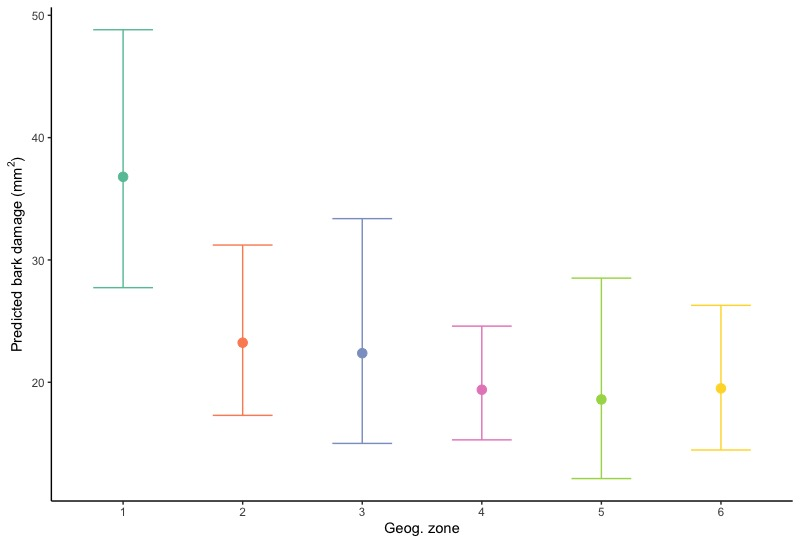
\includegraphics[width=\textwidth]{pred_lmer}
	\caption{Predicted values of mm\textsuperscript{2} for saplings with seed collected from different Geographic Zones.}
\end{figure}

\begin{figure}
	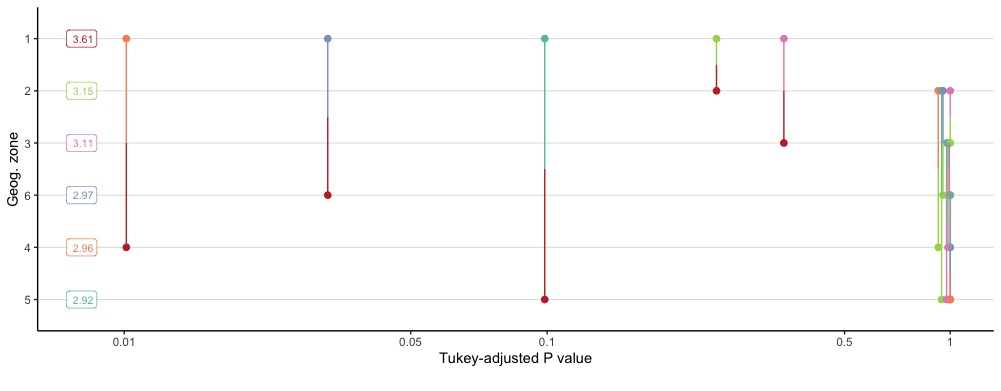
\includegraphics[width=\textwidth]{marginal_means}
	\caption{Pairwise p-values of a Tukey HSD test comparing geographic zones in the best model predicting variation in bark area damaged by \textit{H. abietis}. Geographic zone 1 is significantly (p\textless{}0.05) different from zones 6 and 4. P-values for all other comparisons outwith Geographic zone 1 are close to 1.}
\end{figure}

\begin{table}
	\centering 
	\caption{Model comparison of Generalised Linear Mixed Effects models predicting the area of bark damaged, for those saplings which were damaged. Models are ordered by increasing AIC value.} 
	\begin{tabular}{@{\extracolsep{5pt}} cccc} 
	\hline \\[-1.8ex] 
	\end{tabular} 
	\label{area_comp} 
\end{table} 

% Table created by stargazer v.5.2.2 by Marek Hlavac, Harvard University. E-mail: hlavac at fas.harvard.edu
% Date and time: Mon, Aug 05, 2019 - 11:16:03
\begin{table}[!htbp] 
  \caption{} 
  \label{} 
\centering
\begin{tabular}{@{\extracolsep{5pt}} llS[table-format=3.2]S[table-format=3.2]S[table-format=3.2]S[table-format=3.2]} 
\\[-1.8ex]\hline 
\hline \\[-1.8ex] 
Fixed eff. & Random eff. & {AIC} & {logLik} & {R\textsuperscript{2}\textsubscript{m}} & {R\textsuperscript{2}\textsubscript{c}} \\ 
\hline \\[-1.8ex] 
Geog. zone & Site & 719.471 & -351.735 & 0.056 & 0.056 \\ 
NA & NA & 721.787 & -358.893 & 0 & 0 \\ 
NA & Geog. zone / Site & 722.193 & -357.096 & 0 & 0.033 \\ 
NA & Site / Family & 724.929 & -358.464 & 0 & 0.026 \\ 
Site & Geog. zone & 736.127 & -345.063 & 0.106 & 0.106 \\ 
Site & Family & 736.127 & -345.063 & 0.106 & 0.106 \\ 
Site & Geog. zone + Family & 738.127 & -345.063 & 0.106 & 0.106 \\ 
Family & Geog. zone & 810.131 & -256.066 & 0.565 & 0.565 \\ 
Family & Geog. zone / Site & 812.131 & -256.066 & 0.565 & 0.565 \\ 
Geog. zone & Site / Family & {NA} & {NA} & 0.056 & 0.056 \\ 
\hline \\[-1.8ex] 
\end{tabular} 
\end{table} 

\todo{How strong was the effect of seed population?}

\todo{Look at which populations are the most different}

\subsection*{Population level spatial patterns}

There was a weak positive but significant effect of latitude on the total bark area damaged by \textit{H. abietis} (Z = 3.249(1, 248), p =  \textless{}0.005, R\textsuperscript{2} = 0.041), when the nested random effects of seed collection site and family were accounted for (Figure \ref{latitude}). In a similar model, there was no effect of longitude on bark area damaged (Z = -1.377(1, 248), p = 0.168, R\textsuperscript{2} = 0.009).  

\begin{figure}
	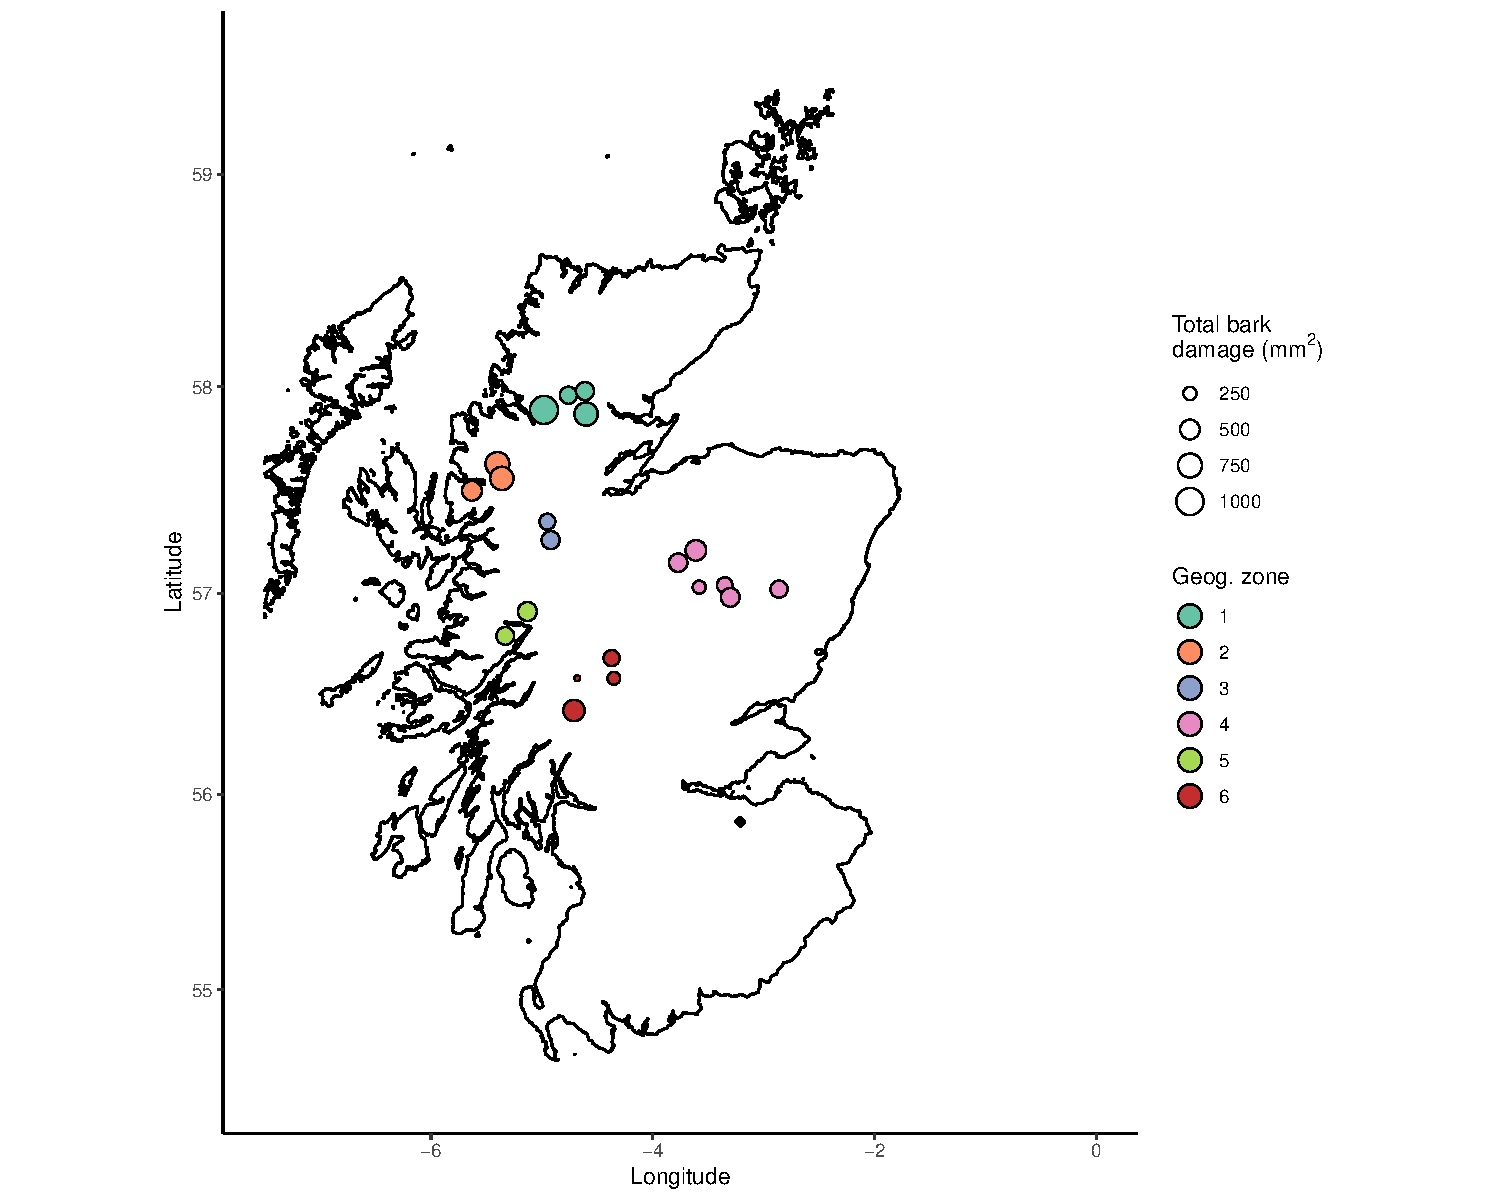
\includegraphics[width=\textwidth]{bubble_map}	
	\caption{Map of study sites}
\end{figure}

\begin{figure}
	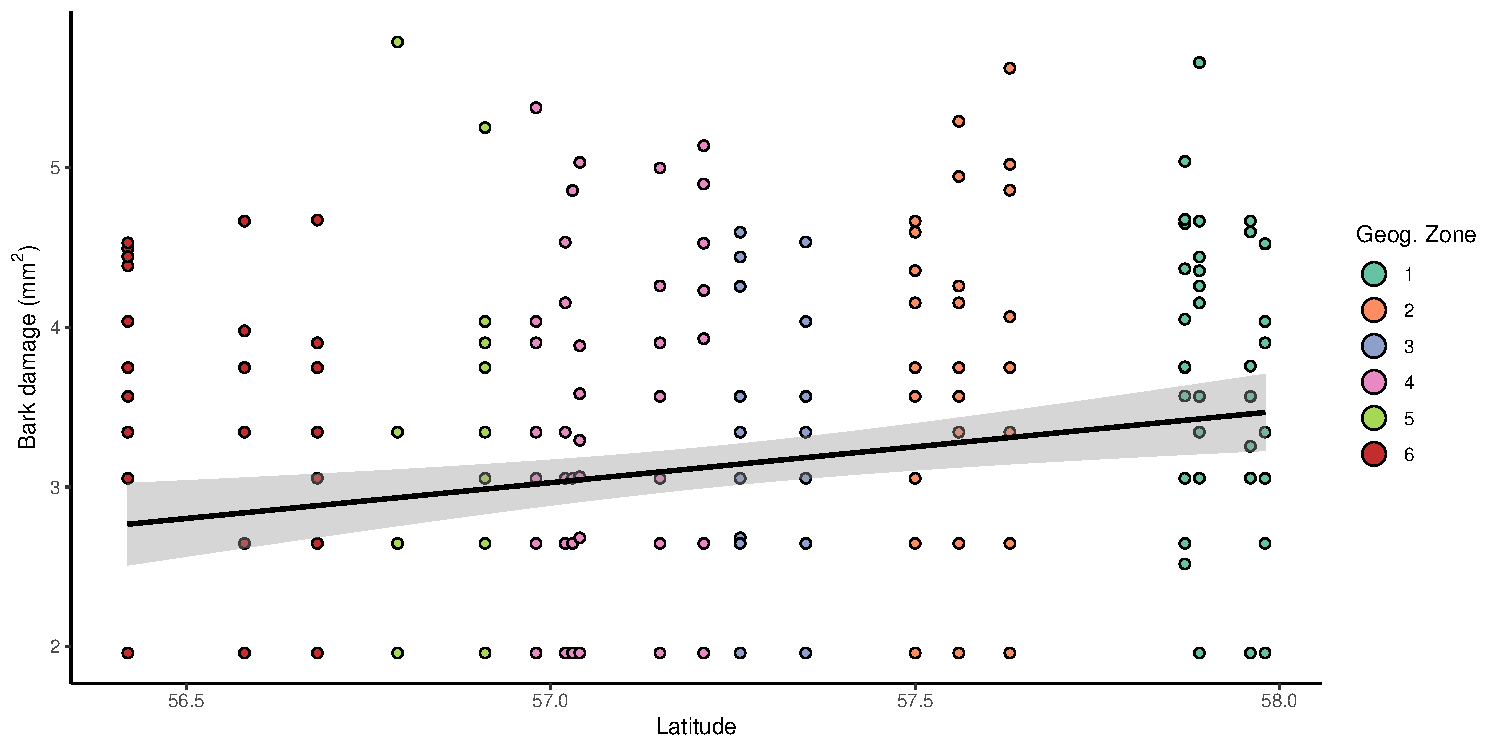
\includegraphics[width=\textwidth]{latitude}
	\caption{Relationship between bark area damaged and latitude of sapling population, for those saplings which were damaged. Each point is an individual sapling. Points are coloured by Geographic zone. The linear model fit (black line with grey 95\% confidence interval) shows a weak positive trend.}
	\label{latitude}
\end{figure}

\begin{figure}
	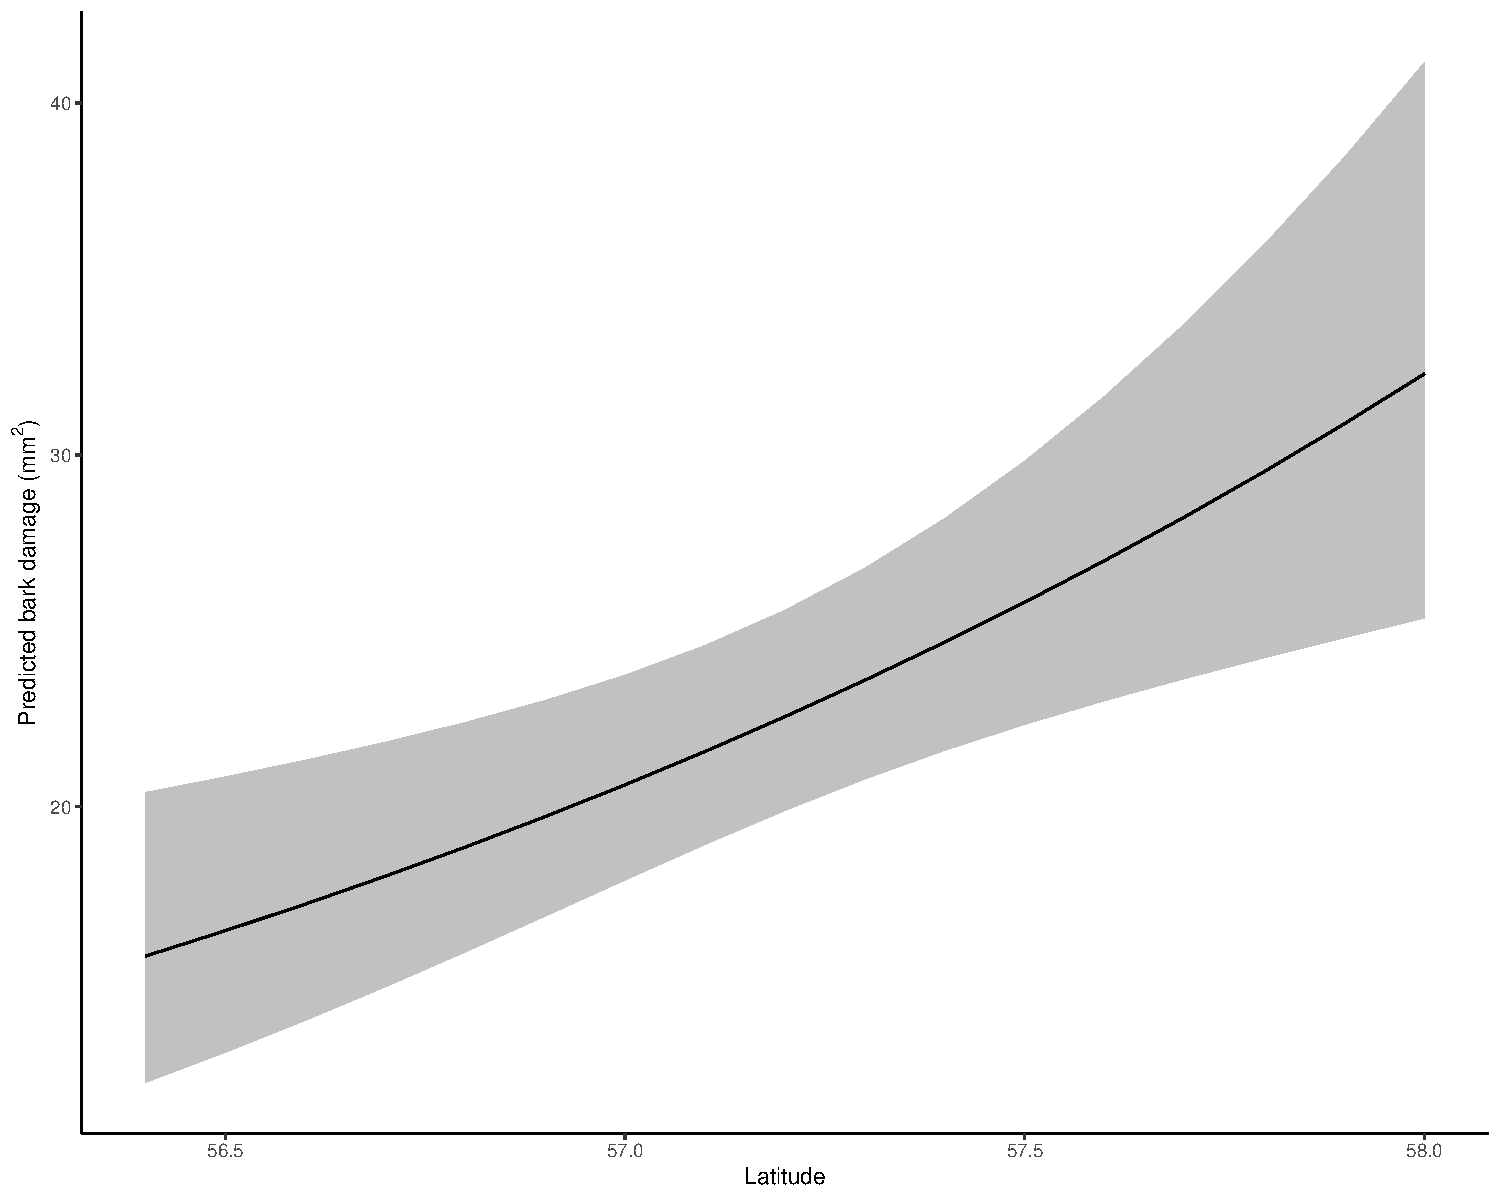
\includegraphics[width=\textwidth]{pred_lat}
	\caption{Predicted values with 95\% confidence interval for the bark area damaged on a sapling when the seed was collected at different latitudes.}
\end{figure}


\subsection*{Parent effects - variation within populations}

Variance in bark area damaged was high in all seed populations. The highest being 216.5 mm\textsuperscript{2} in Cona Glen (Figure \ref{boxplot}).

\section*{Discussion}

The model selection process determined that there was an effect of seed population on the amount of weevil damage found on damaged saplings, but could not account for variation in the probability that a sapling became damaged. Linear models demonstrated that there was a general latitudinal effect on sapling damaged area, with saplings with parents at higher latitudes typically experiencing higher levels of damage, but this had much less effect than population itself. Studies on the distribution and life cycle of \textit{H. abietis} have shown that life cycle length is strongly linked with mean temperature in the summer months, with higher temperatures leading to a short life cycle and therefore higher numbers of pine weevils where infestations occur \citep{Leather1999}. \textit{H. abietis} abundance reduces with latitude in Scotland \citep{Barredo2015}. The latitudinal effect may therefore be a result of adaptation to resist \textit{H. abietis} damage. \textit{P. sylvestris} leaves and bark have resin canals which act to deter herbivores \citep{}. While it has not been explicitly tested for \textit{H abietis}, other studies involving \todo{SOME INSECTS} have found a negative correlation between resin canal density in leaves and feeding behaviour for \textit{P. sylvestris}. \citet{} found that \textit{H. abietis} was discouraged from eating \todo{tree name} needles with higher resin canal concentration and cuticle thickness.

Within population variability was high. \todo{This is expected given the high gene flow}. The effect of population was higher however.

Other things that might have caused variation among seed populations \todo{dunno}.


\section*{Conclusion}

This study sought to test whether adaptive variation for resistance to the large pine weevil (\textit{Hylobius abietis}) existed in genetically distinct populations of scot's pine (\textit{Pinus sylvestris}) in Caledonian remnant forest patches in Scotland. A weak positive effect of latitude of seed collection site was found in the damaged area of sapling bark, suggesting that more southerly populations may be less attractive to \textit{H. abietis} attack. It is suggested that further studies investigate bark morphological variation and concentrations and variation in Volatile Organic Compounds (VOCs) emitted when bark is damaged in young saplings cultivated from seed stock collected from these Caledonian remnant forest patches to understand the underlying mechanism for this variation in attractiveness. 

\bibliography{weevils}

%-----------------------------------------------
\end{document}
%-----------------------------------------------


% Think about framing the question in terms of identifying conservation priorities for genetically distinct populations which don't have much resistance to the weevils
% Alright idea, but natural population of scots pine really don't have that much damage from pine weevils, mainly because there aren't an abundance of stumps and young trees close together in natural populations.


%Gershenzon, J., Croteau, R., 1991. Terpenoids. In: Rosenthal, G.A., Berenbaum, M.R. (Eds.), Herbivores, their Interactions with Secondary Plant Metabolites. Aca- demic Press, New York, pp. 165–219.
